\documentclass[11pt]{article}
\usepackage[a4paper,top=0.6cm,bottom=3.0cm,left=1.8cm,right=1.8cm,footskip=2.0cm]{geometry}
\usepackage{graphicx}
\usepackage[table]{xcolor}
\usepackage{ragged2e}
\usepackage{array}
\usepackage{fancyhdr}
\usepackage{fontspec}
\setmainfont{Tiro Devanagari Hindi}
\setsansfont{Tiro Devanagari Hindi}
\newfontfamily\latinfont{Carlito}
\renewcommand{\familydefault}{\sfdefault}
\definecolor{titleblue}{HTML}{0F2F4A}
\definecolor{textblack}{HTML}{1A1A1A}
\definecolor{rule}{HTML}{C9C4C0}
\definecolor{muted}{HTML}{6B635E}
\definecolor{rowalt}{HTML}{F3F1EF}
\setlength{\parindent}{0pt}\setlength{\parskip}{0.5em}

\setlength{\headheight}{28pt}\setlength{\headsep}{6pt}
\newcommand{\idmfooter}{%
  \begin{minipage}{\textwidth}
    {\color{rule}\hrule height 0.7pt}\vspace{4pt}
    \noindent
    \begin{minipage}[c]{0.66\textwidth}{\scriptsize\color{muted}{\latinfont Developed by the Water and Climate Lab, IIT Gandhinagar. Forecasts are driven by an extended-range forecast system}.}\end{minipage}\hfill
    \begin{minipage}[c]{0.32\textwidth}\raggedleft
      
\includegraphics[height=0.62cm]{wcl.png}\hspace{6pt}%
      
\includegraphics[height=0.62cm]{iitgn.png}
    \end{minipage}\\[3pt]
    {\scriptsize\color{muted}© {\latinfont 2026 Water and Climate Lab} · {\latinfont Indian Institute of Technology Gandhinagar} · {\latinfont For research and demonstration purposes}.}
  \end{minipage}%
}
\newcommand{\idmrunhead}{%
  \begin{minipage}{\textwidth}
    {\small\bfseries\color{titleblue}{\latinfont Drought (CDI) Forecast Outlook}}\hfill{\small\color{muted}{\latinfont Forecast initialized May 20, 2026}  ·  {\latinfont valid through Jun 19, 2026}}\\[2pt]
    {\color{rule}\hrule height 0.6pt}
  \end{minipage}%
}
\fancypagestyle{idmfoot}{\fancyhf{}\renewcommand{\headrulewidth}{0pt}\renewcommand{\footrulewidth}{0pt}\fancyfoot[C]{\idmfooter}}
\fancypagestyle{idmrun}{\fancyhf{}\renewcommand{\headrulewidth}{0pt}\renewcommand{\footrulewidth}{0pt}\fancyhead[C]{\idmrunhead}\fancyfoot[C]{\idmfooter}}
\pagestyle{idmrun}

\begin{document}

\thispagestyle{idmfoot}
\noindent
\begin{minipage}[c]{0.16\textwidth}
\includegraphics[width=\linewidth]{wcl.png}\end{minipage}\hfill
\begin{minipage}[c]{0.80\textwidth}\raggedleft
  {\fontsize{18}{21}\selectfont\bfseries\color{titleblue}{\latinfont Drought (CDI) Forecast Outlook}}\\[2pt]
  {\normalsize\color{muted}{\latinfont Forecast initialized May 20, 2026}  ·  {\latinfont valid through Jun 19, 2026}}
\end{minipage}
\vspace{6pt}{\color{rule}\hrule height 1pt}\vspace{10pt}
{\large\bfseries\color{titleblue}{\latinfont Forecast maps (7 / 15 / 30 day)}}\\[4pt]
\noindent
\begin{minipage}[t]{0.323\textwidth}\centering{\small\bfseries\color{muted}{\latinfont 7-day}}\\[2pt]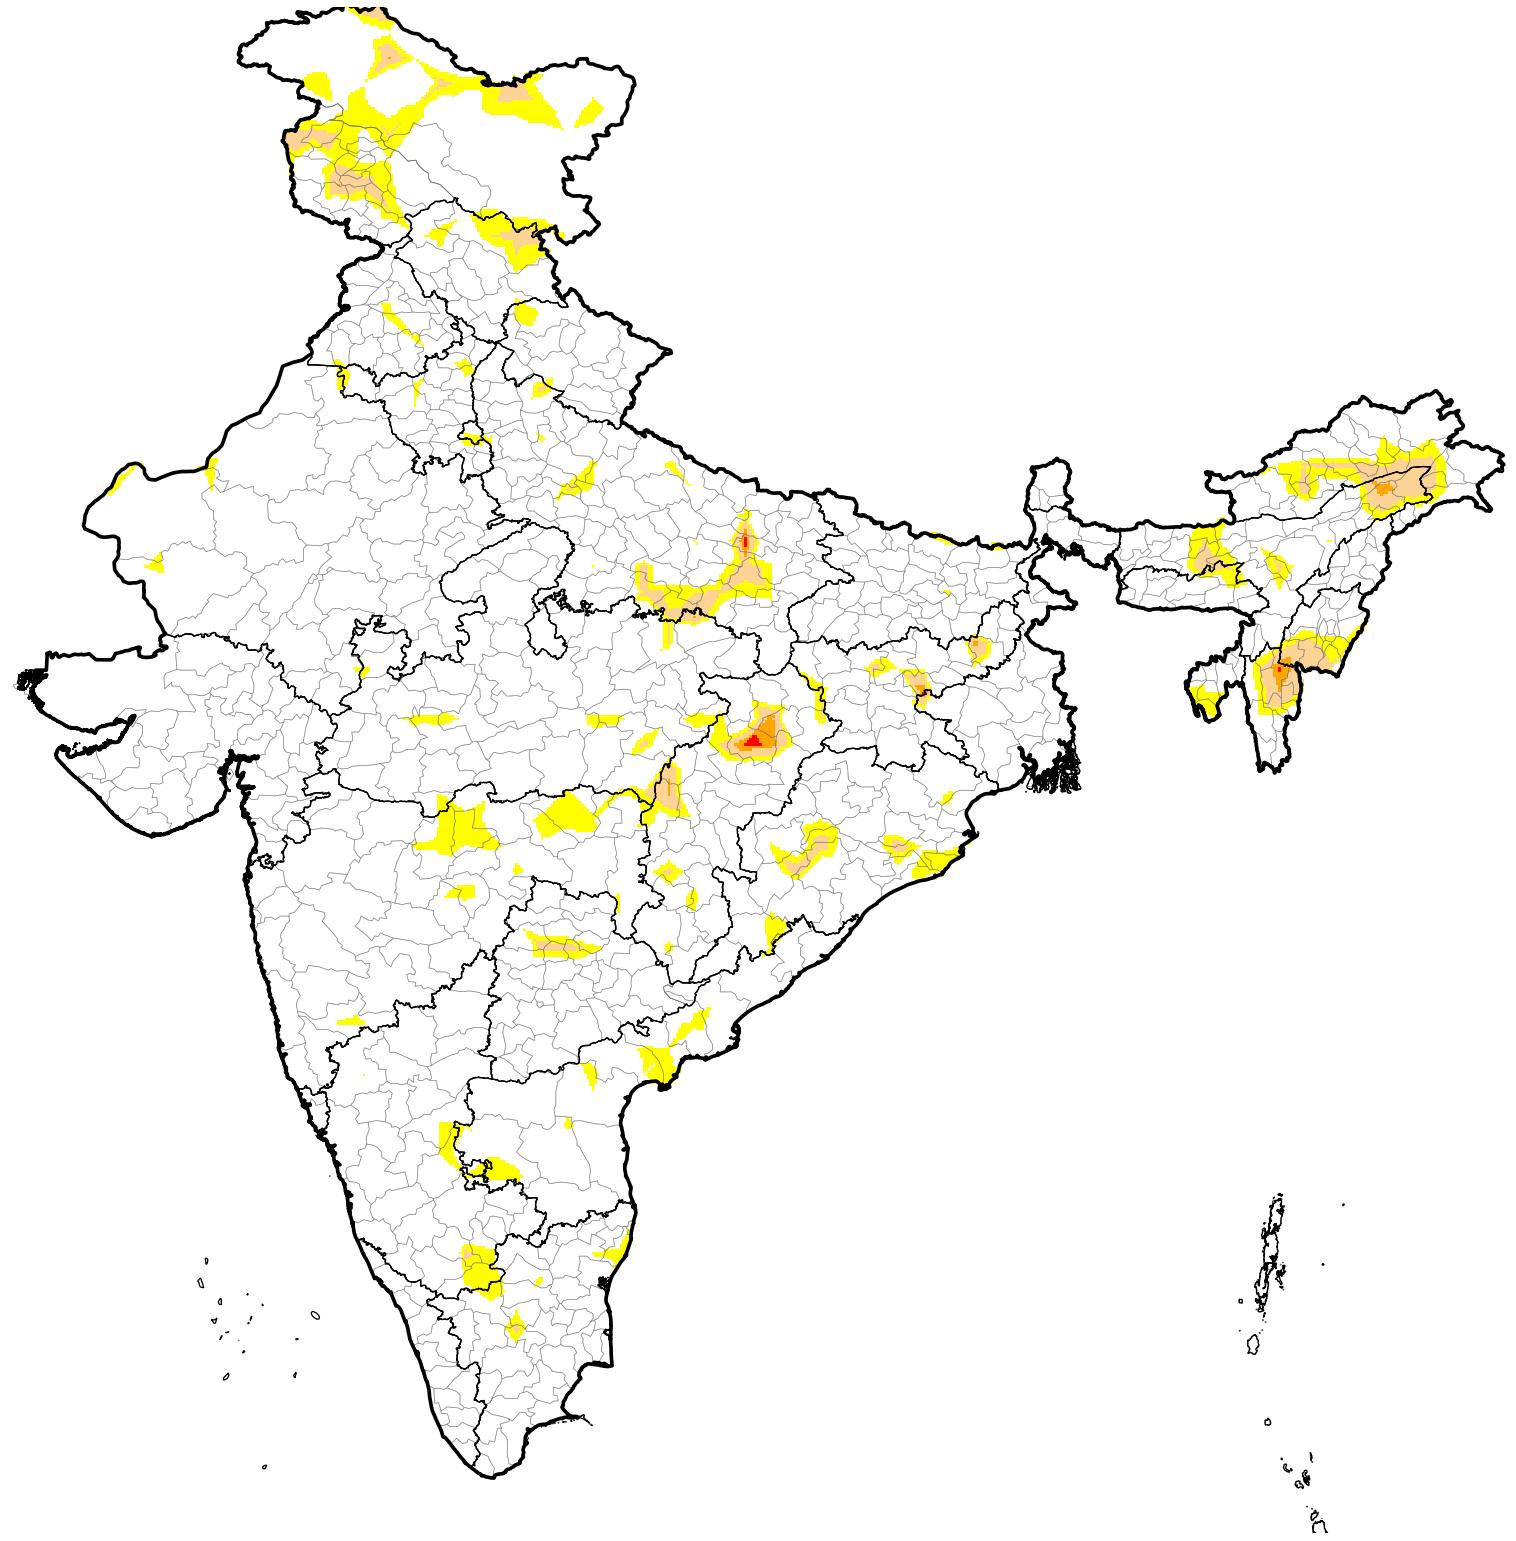
\includegraphics[width=\linewidth]{map7.png}\end{minipage}\hfill
\begin{minipage}[t]{0.323\textwidth}\centering{\small\bfseries\color{muted}{\latinfont 15-day}}\\[2pt]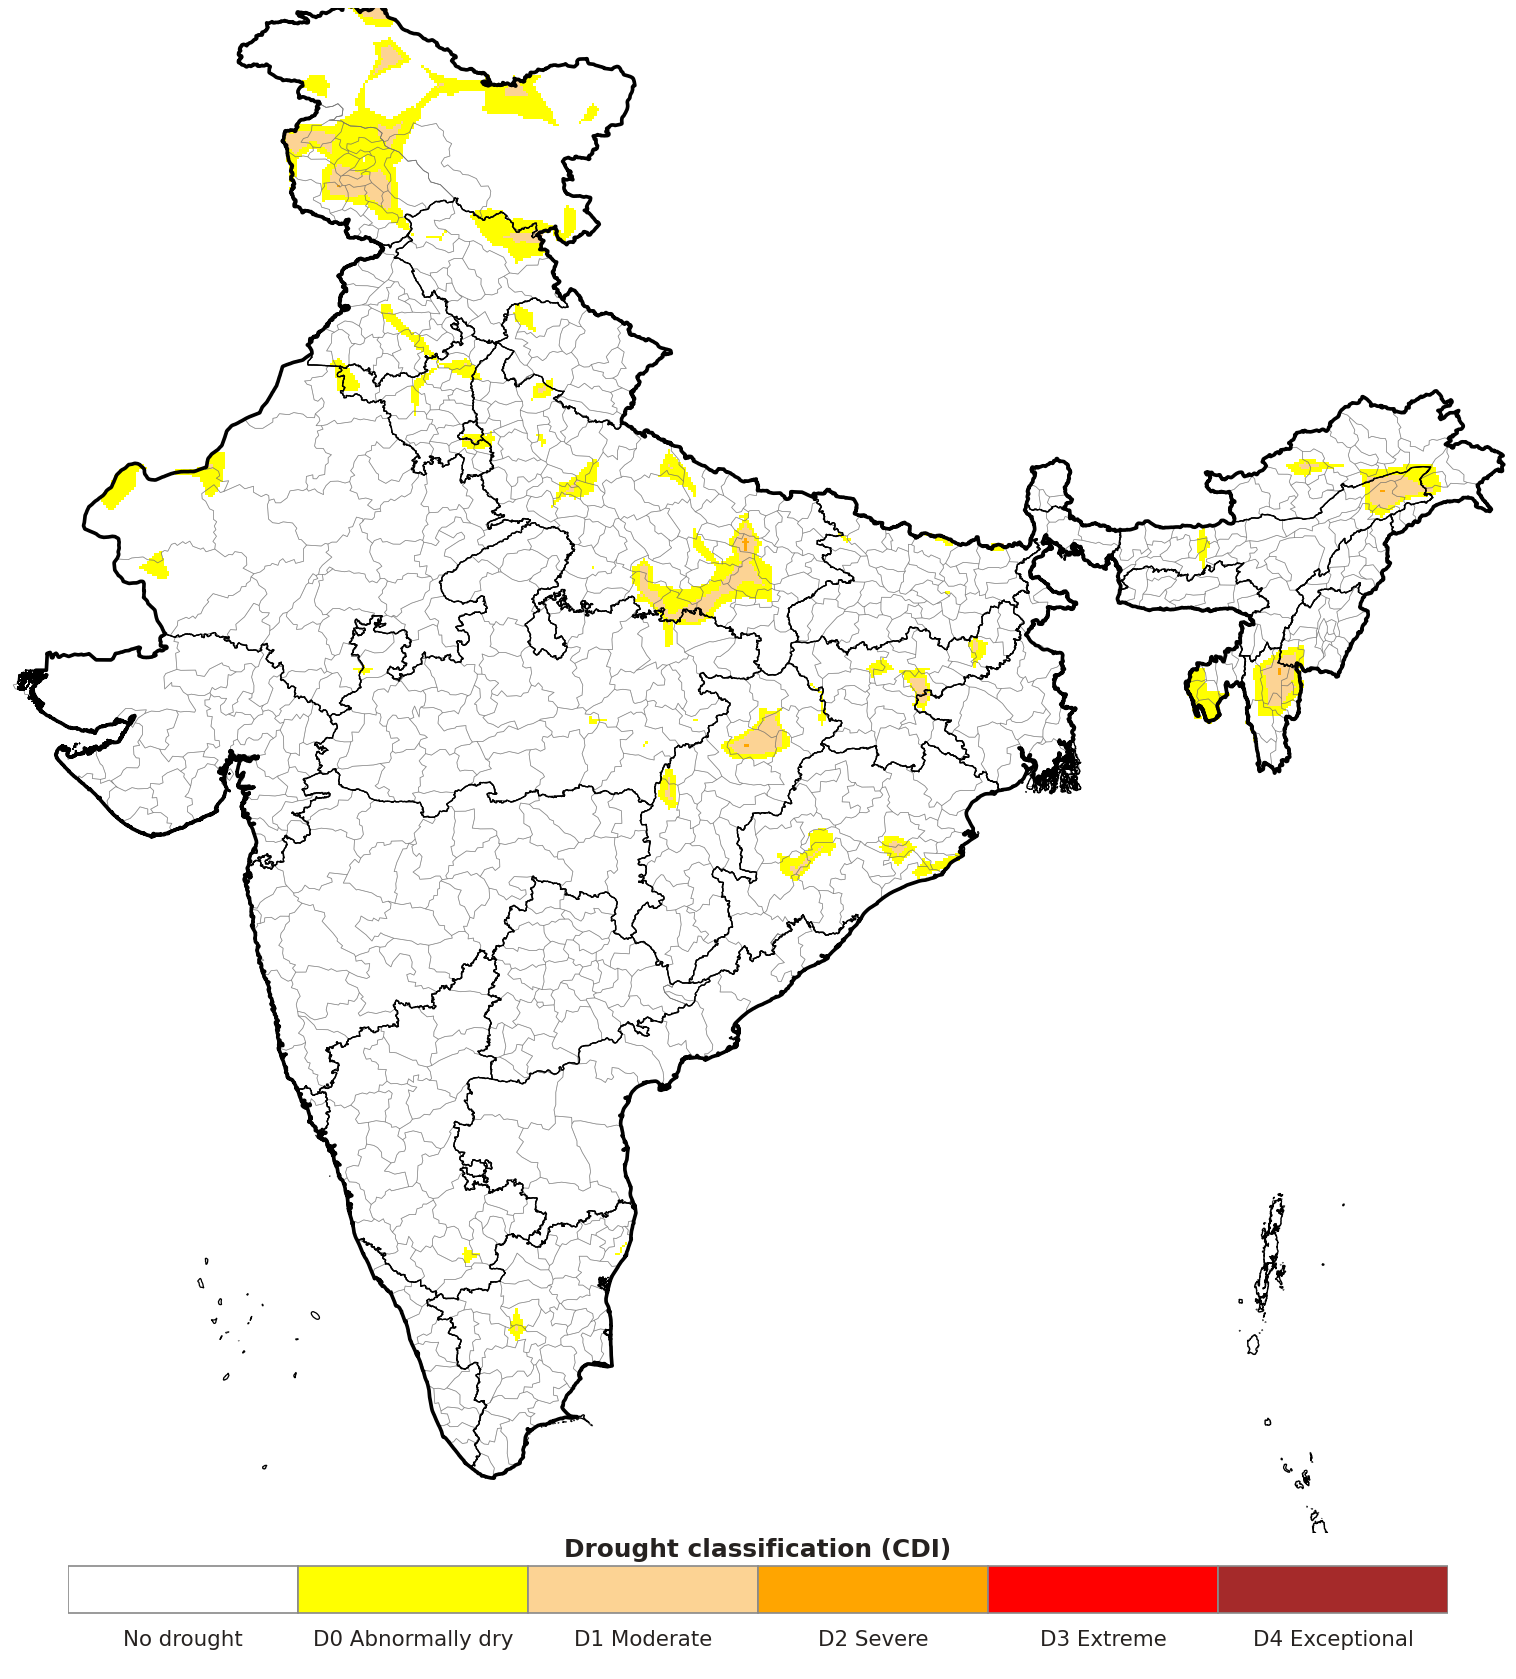
\includegraphics[width=\linewidth]{map15.png}\end{minipage}\hfill
\begin{minipage}[t]{0.323\textwidth}\centering{\small\bfseries\color{muted}{\latinfont 30-day}}\\[2pt]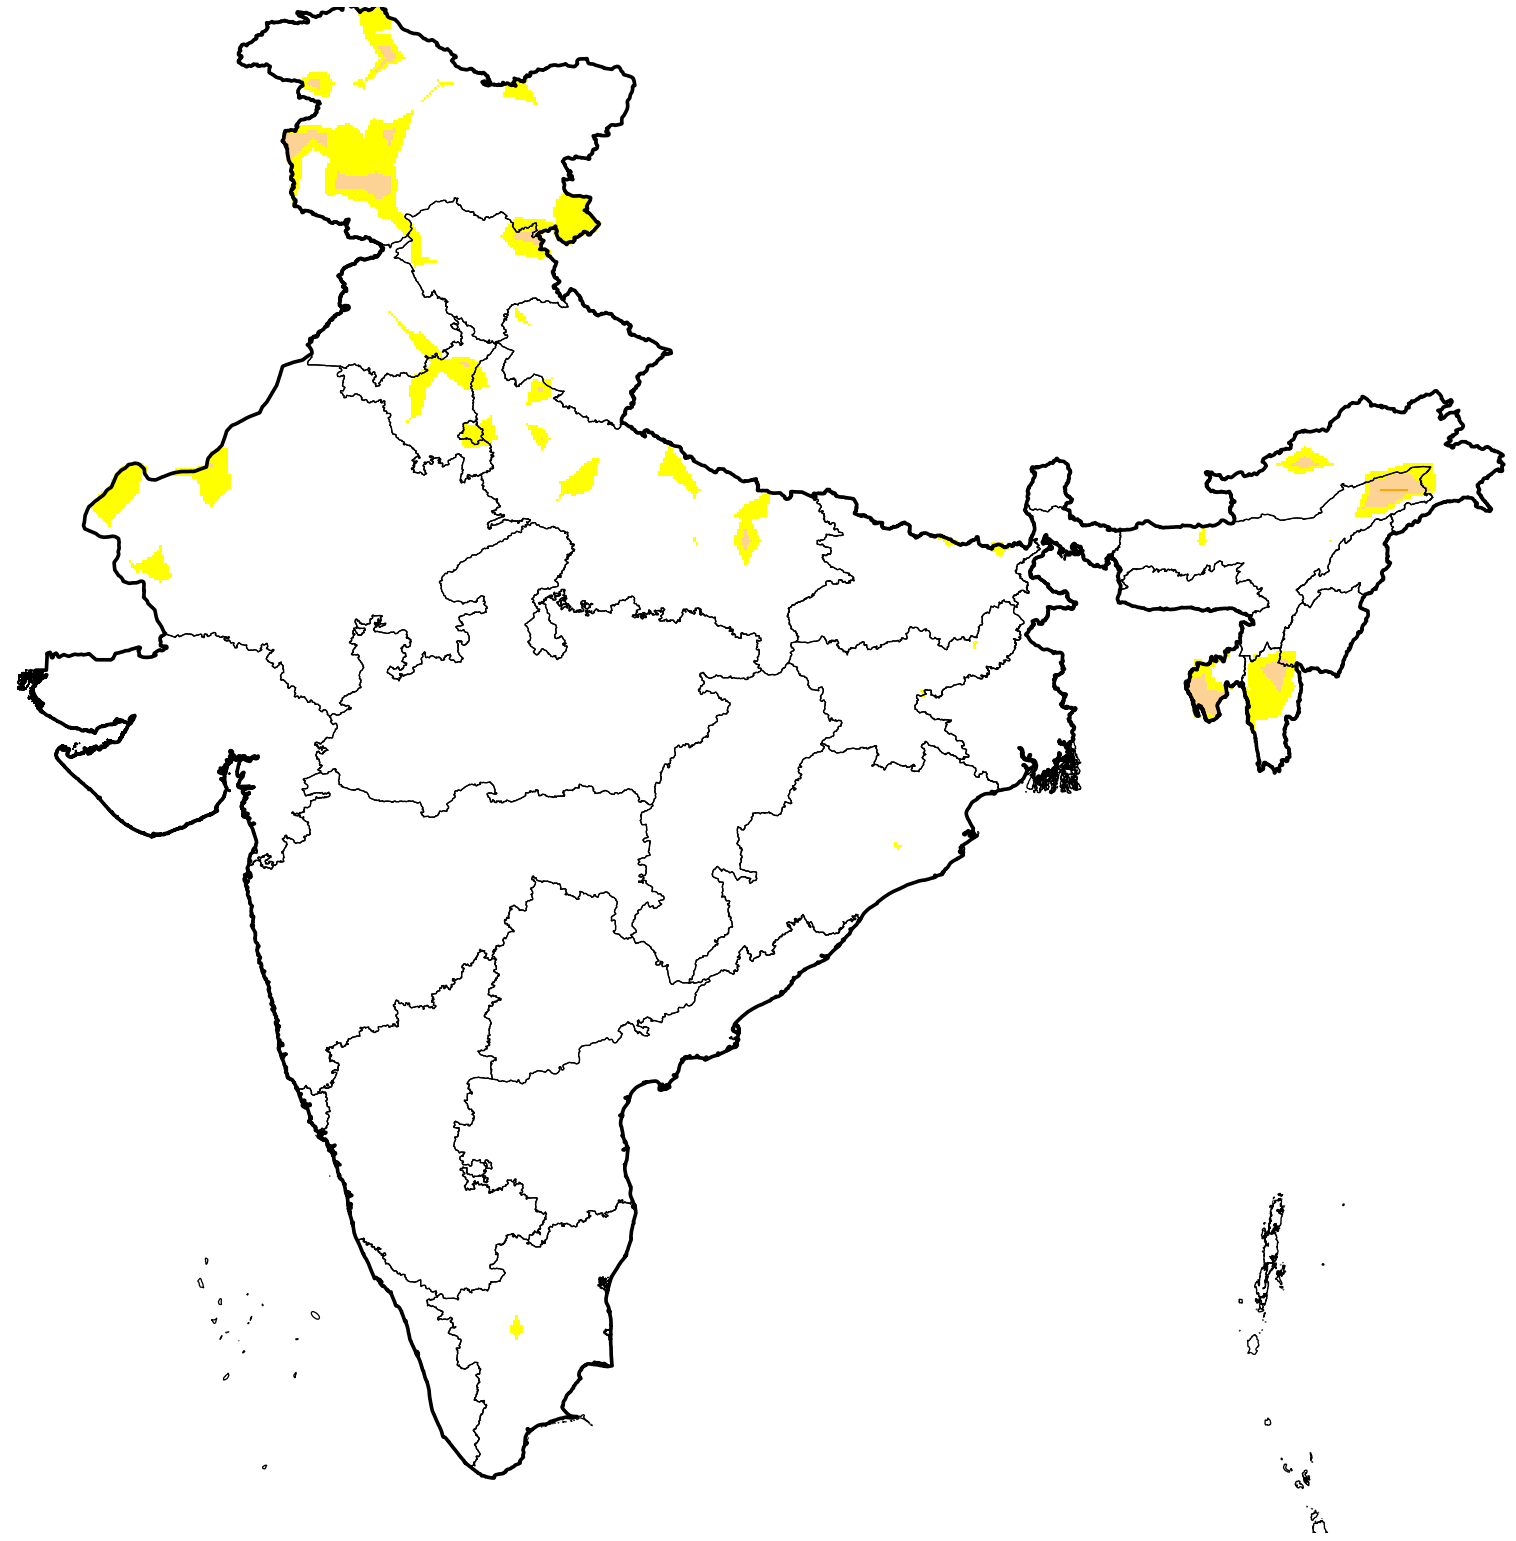
\includegraphics[width=\linewidth]{map30.png}\end{minipage}
\\[3pt]{\small\color{muted}{\latinfont Forecast drought (cdi) for the 7-, 15- and 30-day horizons, initialized May 20, 2026}.}\par
\vspace{10pt}
{\large\bfseries\color{titleblue}{\latinfont Outlook}}\\[2pt]
{\justifying\normalsize\color{textblack}सूखे का पूर्वानुमान (डी{\latinfont 0} से डी{\latinfont 4) 7} दिनों में भारत के लगभग {\latinfont 14} प्रतिशत, {\latinfont 15} दिनों में {\latinfont 10} प्रतिशत और {\latinfont 30} दिनों में {\latinfont 6} प्रतिशत को कवर करने की उम्मीद है।\par}
\vspace{8pt}
{\large\bfseries\color{titleblue}{\latinfont Regional Outlook}}\\[3pt]
{\normalsize\color{muted}{\latinfont Forecast drought area} (\% {\latinfont of region in D0}–{\latinfont D4)}}\\[4pt]
\renewcommand{\arraystretch}{1.3}
\begin{tabular}{@{}p{0.30\textwidth} >{\raggedleft\arraybackslash}p{0.16\textwidth} >{\raggedleft\arraybackslash}p{0.16\textwidth} >{\raggedleft\arraybackslash}p{0.16\textwidth}@{}}
\rowcolor{titleblue}
\textcolor{white}{\textbf{ {\latinfont Region} }} & \textcolor{white}{\textbf{ {\latinfont 7-day} }} & \textcolor{white}{\textbf{ {\latinfont 15-day} }} & \textcolor{white}{\textbf{ {\latinfont 30-day} }}\\
\rowcolor{rowalt} {\latinfont North} & {\latinfont 22} & {\latinfont 26} & {\latinfont 16}\\
 {\latinfont Northwest} & {\latinfont 5} & {\latinfont 6} & {\latinfont 7}\\
\rowcolor{rowalt} {\latinfont Northeast} & {\latinfont 31} & {\latinfont 17} & {\latinfont 20}\\
 {\latinfont East} & {\latinfont 10} & {\latinfont 8} & {\latinfont 2}\\
\rowcolor{rowalt} {\latinfont Central} & {\latinfont 15} & {\latinfont 8} & {\latinfont 0}\\
 {\latinfont West} & {\latinfont 14} & {\latinfont 0} & {\latinfont 0}\\
\rowcolor{rowalt} {\latinfont South} & {\latinfont 11} & {\latinfont 1} & {\latinfont 0}\\
\end{tabular}
\end{document}
